\subsection{垂线}\label{subsec:czjh1-2-2}

我们研究两条相交直线的特殊情形。

如图 \ref{fig:czjh1-2-3} , 直线 $AB$、$CD$ 相交于点 $O$,$\angle BOC$ 为直角。
根据邻补角的性质与对顶角的性质,可以知道,
其他三个角 $\angle AOC$、$\angle BOD$、$\angle AOD$ 都是直角。

当两条直线相交所构成的四个角中有一个是直角时,我们说这\zhongdian{两条直线互相垂直},
其中的一条直线叫做另一条直线的\zhongdian{垂线}。它们的交点叫做\zhongdian{垂足}。

垂直用符号 “$\perp$” 表示,两条直线 $AB$ 与 $CD$ 垂直,
记作 $AB \perp CD$ (或 $CD \perp AB$),读作 “$AB$ 垂直于 $CD$”。
如果垂足为 $O$,写作 “$AB \perp CD$, 垂足为 $O$” (图 \ref{fig:czjh1-2-3})。

如图 \ref{fig:czjh1-2-3}, 已知 $\angle BOC = 90^\circ$,根据垂直的定义,可以得出 $AB \perp CD$;
反过来,已知 $AB \perp CD$,那么根据垂直的定义可得出 $\angle BOC = \angle AOC = \angle AOD = \angle BOD = 90^\circ$。

\begin{figure}[htbp]
    \centering
    \begin{minipage}[b]{4cm}
        \centering
        \begin{tikzpicture}
	\pgfmathsetmacro{\r}{1.5}
	\pgfmathsetmacro{\a}{45}
	\tkzDefPoints{0/0/O}
	\tkzDefPoint(\a:\r){C}
	\tkzDefPoint(90+\a:\r){A}
	\tkzDefPoint(180+\a:\r){D}
	\tkzDefPoint(270+\a:\r){B}

	\tkzDrawSegments(A,B  C,D)
	\tkzMarkRightAngle(B,O,C)
	\tkzLabelPoints[below](A,B,C,D)
	\tkzLabelPoints[left](O)
\end{tikzpicture}


        \caption{}\label{fig:czjh1-2-3}
    \end{minipage}
    \qquad
    \begin{minipage}[b]{4cm}
        \centering
        \begin{tikzpicture}[scale=0.8]
	\tkzDefPoints{0/0/A, 4/0/B, 0.5/-1.5/C, 3.5/1.5/D}
	\tkzInterLL(A,B)(C,D)   \tkzGetPoint{O}

	\tkzDrawSegments(A,B  C,D)
	\tkzLabelPoints[below](A,O,B)
	\tkzLabelPoints[right](C,D)
\end{tikzpicture}


        \caption{}\label{fig:czjh1-2-4}
    \end{minipage}
    \qquad
    \begin{minipage}[b]{5cm}
        \centering
        \begin{tikzpicture}[scale=0.8]
	\tkzDefPoints{-2/0/A, 2/0/B, 0/-1.5/C, 0/1.5/D}
	\tkzInterLL(A,B)(C,D)   \tkzGetPoint{O}

	\tkzDrawSegments(A,B  C,D)
	\tkzMarkRightAngle(B,O,D)
	\tkzLabelSegment[pos=1.0, right](A,B){水平线}
	\tkzLabelSegment[pos=1.0, above](C,D){垂直线}
\end{tikzpicture}


        \caption{}\label{fig:czjh1-2-5}
    \end{minipage}
\end{figure}

两条直线相交不成直角时,其中的一条叫做另一条的\zhongdian{斜线},它们的交点叫做\zhongdian{斜足}。
如图 \ref{fig:czjh1-2-4}, 直线 $CD$ 是 $AB$ 的斜线, $AB$ 也是 $CD$ 的斜线,点 $O$ 是斜足。

在生产和生活中,常常遇到两条直线互相垂直的情形。
例如,水平线和铅垂线是互相垂直的(图 \ref{fig:czjh1-2-5}),
黑板的相邻的两条边、篮球场地的相邻两条边线也都是互相垂直的。

\begin{figure}[htbp]
    \centering
    \begin{minipage}[b]{7cm}
        \centering
        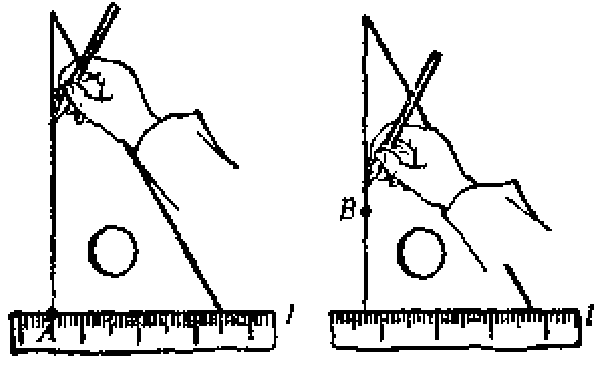
\includegraphics[width=6cm]{../pic/czjh1-ch2-06.png}
        \caption{}\label{fig:czjh1-2-6}
    \end{minipage}
    \qquad
    \begin{minipage}[b]{7cm}
        \centering
        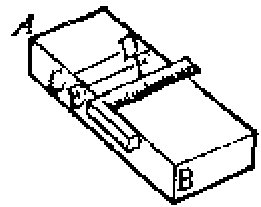
\includegraphics[width=4cm]{../pic/czjh1-ch2-07.png}
        \caption{}\label{fig:czjh1-2-7}
    \end{minipage}
\end{figure}

经过已知直线 $l$ 上的一点 $A$ 或直线 $l$ 外一点 $B$ 画直线 $l$ 的垂线,可以用三角板或量角器。
用三角板画垂线的方法如图 \ref{fig:czjh1-2-6} 所示。工人师傅在画工件边缘的垂线时,常用角尺(图\ref{fig:czjh1-2-7}) 。

\begin{figure}[htbp]
    \centering
    \begin{minipage}[b]{7cm}
        \centering
        \begin{tikzpicture}
	\tkzDefPoints{-2/0/A, 2/0/B, 0/0/C, 0/2/D, 0/0/P}

	\tkzDrawSegments(A,B  C,D)
	\tkzMarkRightAngle(B,O,D)
	\tkzLabelSegment[pos=0.0, left](A,B){$l$}
	\tkzDrawPoint[fill=black](P)
	\tkzLabelPoints[below](P)
\end{tikzpicture}


        \caption*{甲}
    \end{minipage}
    \qquad
    \begin{minipage}[b]{7cm}
        \centering
        \begin{tikzpicture}
	\tkzDefPoints{-2/0/A, 2/0/B, 0/0/C, 0/2/D, 0/1/P}

	\tkzDrawSegments(A,B  C,D)
	\tkzMarkRightAngle(B,O,D)
	\tkzLabelSegment[pos=0.0, left](A,B){$l$}
	\tkzDrawPoint[fill=black](P)
	\tkzLabelPoints[right](P)
\end{tikzpicture}


        \caption*{乙}
    \end{minipage}
    \caption{}\label{fig:czjh1-2-8}
\end{figure}

如图 \ref{fig:czjh1-2-8} , 已知一条直线 $l$ 和一点 $P$, 无论是点 $P$ 在直线 $l$ 上(图\ref{fig:czjh1-2-8} 甲),
还是在直线 $l$ 外(图 \ref{fig:czjh1-2-8} 乙),经过点 $P$ 都能画一条直线与直线 $l$ 垂直,
而且也只能画一条与直线 $l$ 垂直。所以,垂线有下面的性质:

\begin{xingzhi}
    经过一点有一条而且只有一条直线垂直于已知直线。
\end{xingzhi}

下面,我们来看图 \ref{fig:czjh1-2-9}。点 $P$ 是直线 $l$ 外的一点, $PO \perp l$,垂足为 $O$;
直线 $PA$,$PB$、 $PC$、 … 与直线 $l$ 交于点 $A$、$B$、$C$、…。
因为过点 $P$ 与直线 $l$ 垂直的直线只有一条,所以,
直线 $PA$,$PB$、 $PC$、 …  \; 都是直线 $l$ 的斜线,点 $A$、$B$、$C$、… \; 都是斜足。
线段 $PO$ 是点 $P$ 到直线 $l$ 的\zhongdian{垂线线};
线段 $PA$、$PB$、$PC$、… 都是点 $P$ 到直线 $l$ 的\zhongdian{斜线段}。

\begin{figure}[htbp]
    \centering
    \begin{minipage}[b]{7cm}
        \centering
        \begin{tikzpicture}
	\tkzDefPoints{-2/0/A, -1/0/B, 0/0/O, 1/0/C, 2/0/D, 0/2/P}

	\tkzDrawLine[add=0.3 and 0.3](A,D)
	\tkzDrawLines[add=0.3 and 0.3](A,P  B,P  O,P  C,P  D,P)
	\tkzLabelLine[pos=1.35,right](A,D){$l$}
	\tkzDrawPoint[fill=black](P)
	\tkzLabelPoints[right](P)
	\tkzLabelPoints[below](A,B)
	\tkzLabelPoints[below right](O)
	\tkzLabelPoints[below right, xshift=0.3em](C)
\end{tikzpicture}


        \caption{}\label{fig:czjh1-2-9}
    \end{minipage}
    \qquad
    \begin{minipage}[b]{7cm}
        \centering
        \begin{tikzpicture}
	\tkzDefPoints{-2/0/A, 2/0/B, 0/1.5/C, 0/-1.5/D}
	\tkzInterLL(A,B)(C,D)   \tkzGetPoint{M}

	\tkzDrawSegments[xianduan={below=0pt}](A,B)
	\tkzDrawSegments(C,D)
	\tkzMarkRightAngle(B,M,C)
	\tkzLabelPoints[below](A,B)
	\tkzLabelPoints[right](C,D)
	\tkzLabelPoints[above left](M)
\end{tikzpicture}


        \caption{}\label{fig:czjh1-2-10}
    \end{minipage}
\end{figure}

我们用两脚规比较垂线段 $PO$ 和斜线段 $PA$、$PB$、$PC$、… 的大小,可以知道,
垂线段 $PO$ 比任何一条斜线段都短。由此得出垂线的又一个性质:

\begin{xingzhi}
    直线外一点与直线上各点连结的所有线段中,垂线段最短。
\end{xingzhi}

这句话可以简单说成:
\begin{xingzhi}
    垂线段最短。
\end{xingzhi}

从直线外一点到这条直线的垂线段的长度,叫做\zhongdian{点到直线的距离}。
例如,图 \ref{fig:czjh1-2-9} 中,垂线段 $PO$ 的长度,就是点 $P$ 到直线 $l$ 的距离。

在图 \ref{fig:czjh1-2-10} 中,过线段 $AB$ 的中点 $M$ 画 $AB$ 的垂线 $CD$,
那么直线 $CD$ 垂直于线段 $AB$,并且平分线段 $AB$。
垂直于一条线段并且平分这条线段的直线,叫做这条线段的\zhongdian{垂直平分线}或\zhongdian{中垂线}。

\begin{lianxi}

\xiaoti{任意画一个锐角 $AOB$,在边 $OA$ 上任意取一个点 $C$,过点 $C$ 用三角板画 $CD \perp OA$, $CE \perp OB$。}

\xiaoti{从直线 $AB$ 外一点 $C$ 到直线 $AB$, 画一条垂线段和任意的三条斜线段。
    分别量出这些垂线段和斜线段的长度(精确到 $1\;\haomi$),看哪一条最短。
}

\xiaoti{量出图中下列距离(精确到 $1\;\haomi$):}
\begin{xiaoxiaotis}

    \xxt{点 $B$ 到直线 $AC$ 的距离;}

    \xxt{点 $C$ 到直线 $AB$ 的距离。}

\end{xiaoxiaotis}

\begin{figure}[htbp]
    \centering
    \begin{minipage}[b]{7cm}
        \centering
        \begin{tikzpicture}
	\tkzDefPoints{0/0/A, 1.5/1.2/B, 4/0/C}

	\tkzDrawLines[add=0.3 and 0.3](A,B  A,C  B,C)

	\tkzLabelPoints[below](A,C)
	\tkzLabelPoints[above](B)
\end{tikzpicture}


        \caption*{(第 3、4 题)}
    \end{minipage}
    \qquad
    \begin{minipage}[b]{7cm}
        \centering
        \begin{tikzpicture}
	\tkzDefPoints{-2/0/A, 2/0/B, 0/1.5/C, 0/-1.5/D}
	\tkzInterLL(A,B)(C,D)   \tkzGetPoint{M}

	\tkzDrawSegments[xianduan={below=0pt}](A,B)
	\tkzDrawSegments(C,D)
	\tkzMarkRightAngle(B,M,C)
	\tkzLabelPoints[below](A,B)
	\tkzLabelPoints[right](C,D)
	\tkzLabelPoints[above left](M)
\end{tikzpicture}


        \caption*{(第 5 题)}
    \end{minipage}
\end{figure}


\xiaoti{用三角板和刻度尺画线段 $AB$、$BC$、$CA$ 的中垂线。}

\xiaoti{填空(如图):}
\begin{xiaoxiaotis}

    \xxt{\begin{tblr}[t]{colsep=0pt}
        $\because$ \quad & $AB \perp CD$,$AM = MB$(已知), \\
        $\therefore$     & \ewkh[3em] 是 \ewkh[3em] 的中垂线(中垂线定义);
    \end{tblr}}

    \xxt{\begin{tblr}[t]{colsep=0pt}
        $\because$ \quad & $CD$ 是 $AB$ 的中垂线, \\
        $\therefore$     & $AB \perp \ewkh[3em]$, $AM = \exdfrac{1}{2} \ewkh[3em]$ (中垂线定义)。
    \end{tblr}}

\end{xiaoxiaotis}

\end{lianxi}

